% vim:set et sw=2 ts=4 tw=72:
% Jun 18, 2017

In order to determine the effectiveness of the merge-tree model on
comprehension and summarization of git repositories, we conducted a user
study on 12 participants. The user study is a mixed-methods study, with
focus on the quantitative aspects in order to capture how effective the
\mt model, if it is, at improving the correctness, accuracy, and time
performance metrics of users when performing summarization tasks. We use
the qualitative questions as a means of determine the preference of the
participants, and what aspects they prefered from each tool.

In this section, we describe the methods used in the user study. This
includes an outline of the tasks, the commit selection, and the user
selection.

\subsection{Questions}
\label{sub:questions}

The questions and tasks are broken down into four groups. The first two
groups are purely quantitative in nature; we begin with conceptual tasks
to understand whether the DAG is capable of providing users with an
understanding of how a commit is merged into the master branch, and
other commits that it is merged with. We continue with summarization
tasks, to quantitatively understand if the \mt model makes a difference
in summarization tasks. The third portion is purely qualitative, to gain
better understanding of whether participants preferred working with the
\mt model in \tool, or working with the DAG in Gitk, and what aspects
they preferred from each tool. The final group of questions is simply to
gain a better understanding of the demographic of our participants.

%TODO: Look at how to form research questions in LaTeX

We have two primary research questions;
\begin{enumerate}
  \item Is the DAG capable of providing the participants with an
    understanding of the repository events that are related to a commit?
  \item Does the \mt model make a difference in summarization tasks?
\end{enumerate}

\textbf{Conceptual Tasks}

The participants were allowed to use Gitk or the git command line tools
to perform these tasks. These tasks are asked in this order, allowing
the user to use their diagram to answer the second two questions. It is
not necessary to use \tool in this portion of the study, as it provides
the answers to these questions directly.

\begin{enumerate}
  \item Draw a diagram of the merge tree, showing how the commit was
    merged into the master branch of the repository
  \item How many individual commits are related to this commit?
  \item How many merges are involved with merging this commit into the
    master branch?
\end{enumerate}

We provide the user with 10 minutes per commit to complete the first
task. The answers to the two other questions in this section are drawn
from the answer in the first task.

\textbf{Summarization Tasks}

For these questions, we randomize the order of the tools, choosing to
either start with \tool or Gitk, to ensure that we do not place a bias
on one tool or another through the experiment. The tasks are broken
into task sets related to the overall goal of the task. The task sets
are shuffled, and the tasks within the task sets are shuffled as well.
Finally, the order of the commits is shuffled. We use the
\verb|random.shuffle| function from python 3.6.1 to perform the
shuffling and presentation of the tasks.

\begin{itemize}
  \item Merge task set
    \begin{itemize}
      \item What is the series of merges involved with merging this
        commit?
      \item What other commits are merged in the same merge tree?
    \end{itemize}

  \item Authors task set
    \begin{itemize}
      \item How many authors are involved with this merge tree?
      \item Who contributed the most changes to this merge tree?
    \end{itemize}

  \item Files task set
    \begin{itemize}
      \item How many files were modified in this merge tree?
      \item Which file had the most changes in this merge tree?
    \end{itemize}

  \item Modules task set
    \begin{itemize}
      \item Which modules doe this merge tree involve?
    \end{itemize}
\end{itemize}

As understanding where the merge begins and ends is vital to answering
the other question, the merge task set will always be the first task set
presented; however, the questions will still be re-ordered within the
task set.

\textbf{User Opinion}

Finally, we ask the user for their opinions on the tools and for some
information about their level of experience with git. This portion of
the study is qualitative and does not rely on either of the tool,
instead attempting to determine which model provided the user with a
better experience.

We ask the following questions in this order;

\begin{enumerate}
  \item Given these tasks again, which tool would you prefer to use?
  \item Which aspects of each tool did you like and why?
  \item How long have you used git?
  \item If you have used git, for what kind of projects? (personal,
    school courses, professional?)
  \item If you have used git, how many commits, files, and contributors
    were involved with the largest repository you have worked with?
\end{enumerate}


\subsection{Commit Selection}
\label{sub:commit_selection}

We chose two commits for use in the study. The order that the commits
are presented is randomized between participants, but the order is kept
consistent through the tasks described in the next subsection.

We use the \tool database, containing commits and merge-tree information
from April 16th 2005 to October 14th, 2014, which corresponds to being
between Linux release 2.6.12-rc3 and Linux 3.17-rc1. \evan{Cite the
  database even more?} We chose the commits based on tree sizes. We
found that a majority of the trees contain at most seven inner commits,
while more than 25\% of the trees contain a single commit. 75\% of the
tree contained up to 51 inner commits and merges, and finally the
largest tree contained 7217 nodes. We chose to work with the trees in
the first and second quartile, as merge trees of sizes between one and
seven, not including the merge into the master branch, make up the
majority of the trees in the database.

From here, we selected one tree from the trees of a single commit at
random. Selecting a commit from that tree is trivial, as there is only
one to choose.

We selected one tree of size seven at random from all trees of size
seven. We placed a restriction the trees, the selected tree must include
at least one internal merge to increase the complexity of the trees
tested. After randomly selecting a tree, we chose in internal commit at
random, using the \verb|random.choice| function in python 3.6.1.

% TODO: Show this paragraph in the introduction
% It is worth noting that in the fourth
% quartile, the size of the tree drops off quickly from the top tree, with
% the next tree containing only 4708 nodes, and the third largest tree
% containing only 2349 commits.

Using this technique, we selected commit
\emph{a3c1239eb59c0a907f8be5587d42e950f44543f8} from the tree containing
a single node (Figure~\ref{fig:commit_1}), which we will refer to as
\comA, and commit \emph{cdbdd1676a5379f1d5cbd4d476f5e349f445befe}, from
the tree containing seven nodes (Figure~\ref{fig:commit_2}), which we
will refer to as \comB.

\begin{figure}[bpt]
  \centering
  
\includegraphics[width=0.08\linewidth]{figures/commits/1-commit.pdf}
  \caption{The first merge tree used in the user study, a merge tree
    containing a single commit}
  \label{fig:commit_1}
\end{figure}

\begin{figure}[bpt]
  \centering
  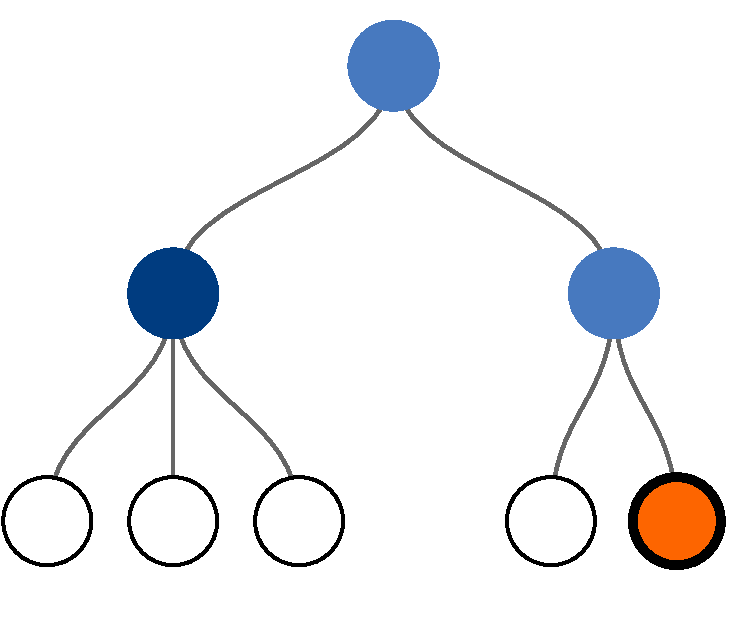
\includegraphics[width=0.5\linewidth]{figures/commits/7-commits.pdf}
  \caption{The second merge tree used in the user study, a merge tree
    containing seven commits}
  \label{fig:commit_2}
\end{figure}


\subsection{User Selection}
\label{sub:user_selection}

Our target audience are git users, particularly users with who are
working on understanding what changes are being made, where they are
being made, and who is making the changes. The merge-tree model is also
intended for users who are trying to learn the structure of a
repository, how modules of the repository are broken into groups, if the

We have software engineering and computer science students at the
Masters, Doctorate, and Post-Doc levels available for participation in
this study. \evan{This feels like the weakest part of the paper, is
  there any way to make it sound stronger?}


\subsection{Data Extraction}
\label{sub:data_extraction}

The study is recorded using screen capture and audio capture software
for further analysis. From the resulting videos, we are able to extract
the timing and accuracy of each participant over each task. We record
the timing, accuracy, task, commit, and tool used for each part. We also
record some addition information about whether the participant was
correct, guessing, partially correct, or completely wrong, as this may
provide some interesting insights.

The answers to each question is relatively straight-forward, as we can
extract the information directly from gitk and Linvis. Measuring the
accuracy of the questions is more challenging. In the question regarding
the merges leading to the merging of a given commit, both the merges and
the ordering of the merges matter. In the cases where the answer is not
a numerical value, we use the edit distance to determine the accuracy of
an answer. An edit distance of zero indicates a correct answer, while
any number other than zero indicates an incorrect answer. Adding,
reordering (where important), and removing commits or merges all incur a
penalty of 1 added to the edit distance.

The correct answers for \comA are shown in
Table~\ref{tab:coma_study_answers}, and the correct answers for \comB are
shown in Table~\ref{tab:comb_study_answers}.

\begin{table}[htpb]
  \centering
  \caption{Answers to the question from the conceptual and summarization portions of the user study for \comA}
  \label{tab:coma_study_answers}
  \begin{tabular}{l|l}
    Question                                              & Answer \\\hline\hline
    Number of commits in the merge tree                   & 1\\
    Number of merges in the merge tree                    & 1\\\hline
    Merges merging this commit into the master branch     & 1 (11df586407)\\
    Other commits that are merged in the same tree        & None\\
    How many authors are involved with this tree?         & 1\\
    Who contributed the most changes to this merge tree   & David\\
    How many files are modified in this merge tree        & 2\\
    Which file(s) had the most changes in this merge tree & both (pzl.c, asl.c)\\
    Which modules does this merge tree involve & wusb
  \end{tabular}
\end{table}


\begin{table}[htpb]
  \centering
  \caption{Answers to the question from the conceptual and summarization portions of the user study for \comB}
  \label{tab:comb_study_answers}
  \begin{tabular}{l|l}
    Question & Answer \\\hline\hline
    Number of commits in the merge tree & 5 \\
    Number of merges in the merge tree & 3\\\hline
    Merges merging this commit into the master branch     & (219b22b245
    \\
    & $\rightarrow$ \\
    & 8eb88c80d4)\\
    Other commits that are merged in the same tree        & ec4e86ba06\\
    & 9a3f371e99\\
    & 1c85cc6445\\
    & 7c2dfee848\\
    How many authors are involved with this tree?         & 4\\
    Who contributed the most changes to this merge tree   & Randy Dunlap\\
    How many files are modified in this merge tree        & 6\\
    Which file(s) had the most changes in this merge tree & pcm\_lib.c\\
    Which modules does this merge tree involve            & ALSA\\
  \end{tabular}
\end{table}

Extracting the timing information is prone to some issues with where the
duration of answering should start and stop. We try to eliminate these
issues by maintaining the following conventions; the answer duration
begins at the end of the last word of the prompt. The duration ends
immediately before the first word of the final modification to the
answer. Many answers are able to be answered in a single word or phrase,
but some may require multiple sentences that are broken by additional
processing by the participant. An Example of questions where the answer
may be interleaved with solving the task is the task asking the user to
provide the merges on the path from the commit into the master branch.
The goal of this is to eliminate the duration required to provide the
prompt, and eliminate the time required to provide the answer.

The information is then inserted into a sql database for further
analysis.

\subsection{Analysis}

As the goals of each section are different, the techniques for analyzing
the results are different. The conceptual questions are to demonstrate
the difficulty in comprehending the DAG model, so we simply provide the
metrics, showing how well the participants did in answering the
questions asked. The summarization tasks are meant for comparing the
ability of the participants to summarize two commits from the Linux
repository. As this is a comparison, further analysis is necessary to
determine the significance of our results. The final portion of the
study is designed to help us understand the group of users that we are
working with.

As the goals of the conceptual questions are to demonstrate the
difficulty in comprehending the DAG model, and determine how closely
users are able to make the mapping from the DAG to showing how a commit
was merged into the master branch, no further statistical analysis will
be performed on this data. We will provide the metrics response,
accuracy, and time metrics for these questions. No comparisons are made
between the models in these tasks, so no further analysis is necessary.

The summarization tasks are designed to compare the two models when the
participant is summarizing various aspects of the repository, including
the files modified and authorship information. We will use three terms
to describe the performance of a user; correctness, which indicates
simply whether the participant was correct or not, making no indication
toward how far from the correct answer they were; accuracy, indicating
how far from the correct answer the participant was; timing, which
indicates how long a participant took to answer the question. We begin
the analysis of these questions using the McNemar test, with $\alpha =
0.005$, measuring the correctness of the results provided by the
participant when using \tool versus gitk.
% TODO: cite the McNemar test maybe?
If the McNemar test indicates that we do not reject the null hypothesis,
we continue analyzing the difference in accuracy and timing metrics for
the merge-tree model versus the DAG.

For each test, we use a confidence level $\alpha = 0.005$, resulting in
a $\chi^2$ test statistic of 7.879.

% TODO: Add the null hypothesis and type of metrics analyzed for each summarization question
